
\chap{Implementation}

\hypersetup{
    colorlinks=true,
    linkcolor=blue,
    filecolor=magenta,      
    urlcolor=blue,
}

\DeclareFixedFont{\ttb}{T1}{txtt}{bx}{n}{12} % for bold
\DeclareFixedFont{\ttm}{T1}{txtt}{m}{n}{12}  % for normal
\definecolor{deepblue}{rgb}{0,0,0.5}
\definecolor{deepred}{rgb}{0.6,0,0}
\definecolor{deepgreen}{rgb}{0,0.5,0}

% Python style for highlighting
\lstset{
	backgroundcolor = \color{Ivory},
    language=Python,
    basicstyle=\footnotesize,
    otherkeywords={self},             
    keywordstyle=\footnotesize\color{deepblue},
    emph={__init__},          
    emphstyle=\footnotesize\color{deepred},    
    stringstyle=\color{deepgreen},
    frame=single,                         
    showstringspaces=false  ,
    breaklines=true,
    numbers=left,
    numberstyle=\footnotesize,
    tabsize=3,
    breakatwhitespace=false
}


\subsection{Implemented Systems repositories}
You can easily download my already implemented system for test it and better understand how it works.

Link for Total implementation Experiment 1 : \\
\url{https://github.com/Sprea22/Data_Analyzer_Python}

Link for Total implementation Experiment 2 : \\
\url{https://github.com/Sprea22/Forecasting_System_Python}

\textbf{How to download and test it:}\\
There are two ways for download it:
\begin{itemize}
\item Download the ZIP files from the following links:\\

Direct link for the already implemented Data Analyzer in Python.\\
\url{https://codeload.github.com/Sprea22/Data_Analyzer_Python/zip/master}\\

Direct link for the already implemented Forecasting System in Python.\\
\url{https://codeload.github.com/Sprea22/Forecasting_System_Python/zip/master}

\newpage
\item If you have already installed github on your computer, you can easily download it creating a folder and then inside that folder open a terminal shell and execute the following commands:\\
\begin{lstlisting}
git init
git remote add origin https://github.com/Sprea22/
		Data\_Analyzer\_Python.git
git pull origin master
\end{lstlisting}

Otherwise:\\

\begin{lstlisting}
git init
git remote add origin https://github.com/Sprea22/
		Forecasting\_System\_Python.git
git pull origin master
\end{lstlisting}
\end{itemize}

Once you downloaded it you will find a readMe inside both the repository that will explain your how to execute and how to test it.

\part{Data collection and validation}
\newpage
\section{Data collection}
\subsection{Data sources}
During this phase of the work the most important thing is to collect as much useful data as possible.The data have been searched on different websites, such as:
\begin{itemize}
\item fiskeridir.no (7 Inputs): \\ This has been the main data source for this work. It provides several statistics about Aquaculture in Norway. The only complications about this website are:
\begin{itemize}
\item XLSX Format: The data are available just in XLSX format, with a lot of comments and county categories.
\item Language: The data are available just in Norwegian.
\item Download: Is not possible to implement a script for automatic download of the data since there isn't a static download link for the latest version.
\item Upload frequency: The data are periodically uploaded once per month.
\end{itemize}

\item indexmundi.com (1 input):\\ Is possible to find data about fish (salmon) monthly price, Norwegian Krone per Kilogram.

\item quandl.com (0 Input):\\ Is possible to find data about fish (salmon) monthly price, US Dollar per Kilogram.

\item kart.fiskeridir.no (0 Input):\\ It allows to show some data about Aquaculture in Norway displayed on a map, and is also possible to download it (not every single data) in XLSX/CSV format. 

\item sildelaget.no (0 Input):\\ This website provides some general statistics about fisheries and also a catch journal.

\end{itemize}


\section{Increase accessibility and availability of data}
Quite complicated datasets structure rebuilt in a easy readable way, provided an accurate description (in English, since it was available just in Norwegian) and collected in a unique big dataset. \\
It allows to access to different kind of values about aquaculture in Norway in a much easier way.

\newpage

\subsection{Data description and validation}
\subsubsection{Dataset about Norway}

\begin{figure}[H]
        \makebox[\textwidth][c]{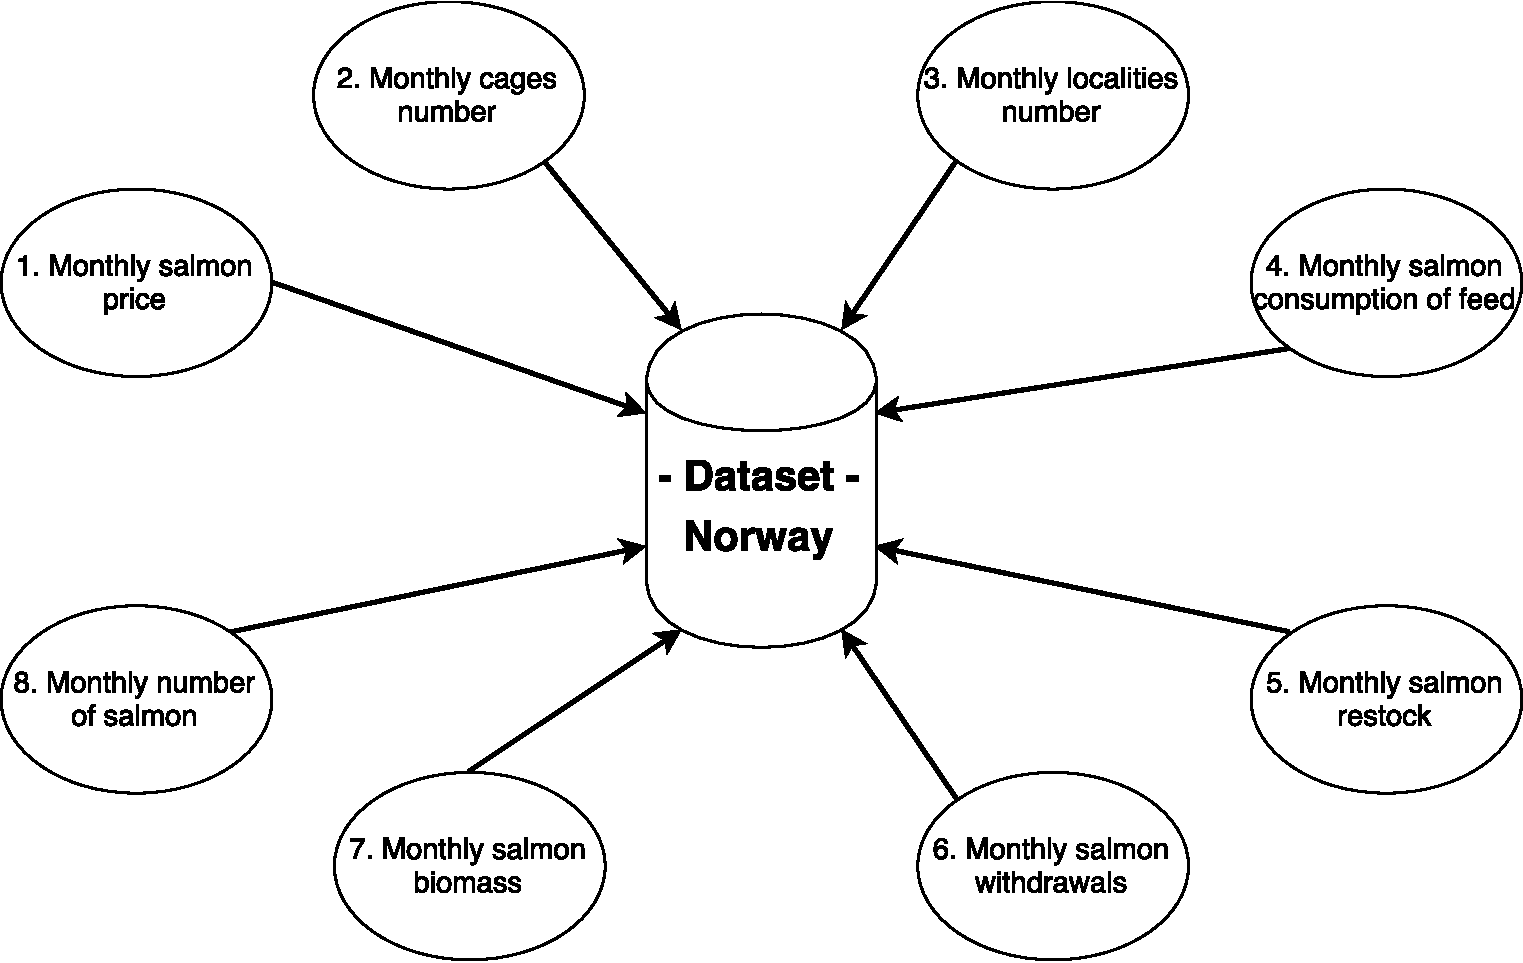
\includegraphics[width=1\textwidth]{Files/Dataset.pdf}}
    \caption{Dataset structure.}
\end{figure}

\makebox[\textwidth][c]{
\resizebox{1.3\textwidth}{!}{
    \begin{tabular}{ | l | l | l | l | l | l | l |}
            \hline
\textbf{Input}							&	\textbf{Content}	& \textbf{Unit} & \textbf{Frequency} & \textbf{Period} & \textbf{Location} & \textbf{Source}	\\ \hline
1. Cages							&	\multicolumn{1}{p{4cm}|}{\raggedright Reported number of cages with salmon and rainbow trout.}
									& Number & Monthly & January 2005 - December 2016 & Norway & 	fiskeridir.no	\\ \hline
									
2. Localities						& \multicolumn{1}{p{4cm}|}{\raggedright Reported number of localities with salmon and rainbow trout.}
									& Number & Monthly & January 2005 - December 2016 & Norway & fiskeridir.no	\\ \hline
3. Monthly\_salmon\_price 			& \multicolumn{1}{p{4cm}|}{\raggedright Fish Salmon, Farm Bred Norwegian Salmon, export price, NOK per kg.}	
									& NOK per kg & Monthly & January 2005 - December 2016 & Norway & 	indexmundi.com	\\ \hline
4. Salmon\_consumption\_of\_feed	&  \multicolumn{1}{p{4cm}|}{\raggedright Reported feed consumption for Salmon.}		
									& Tonnes & Monthly & January 2005 - December 2016 & Norway & 	fiskeridir.no	\\ \hline
5. Salmon\_restock 				& \multicolumn{1}{p{4cm}|}{\raggedright Fish restock reported for Salmon.}	
									& 1000 pcs & Monthly & January 2005 - December 2016 & Norway & 	fiskeridir.no	\\ \hline
6. Salmon\_withdrawals 			& \multicolumn{1}{p{4cm}|}{\raggedright Withdrawals of Salmon for slaughter. } 		
									& Tonnes & Monthly & January 2005 - December 2016 & Norway & 	fiskeridir.no	\\ \hline
7. Salmon\_biomass\_end\_month		& \multicolumn{1}{p{4cm}|}{\raggedright Reported biomass of Salmon. }
									& Tonnes & Monthly & January 2005 - December 2016 & Norway & 	fiskeridir.no	\\ \hline
8. Salmon\_number\_end\_month 		& \multicolumn{1}{p{4cm}|}{\raggedright Reported number of Salmon. }		
									& Number & Monthly & January 2005 - December 2016 & Norway & 	fiskeridir.no	\\ \hline
    \end{tabular}}}
    

\subsubsection{Dataset about each single county} 

\begin{figure}[H]
        \makebox[\textwidth][c]{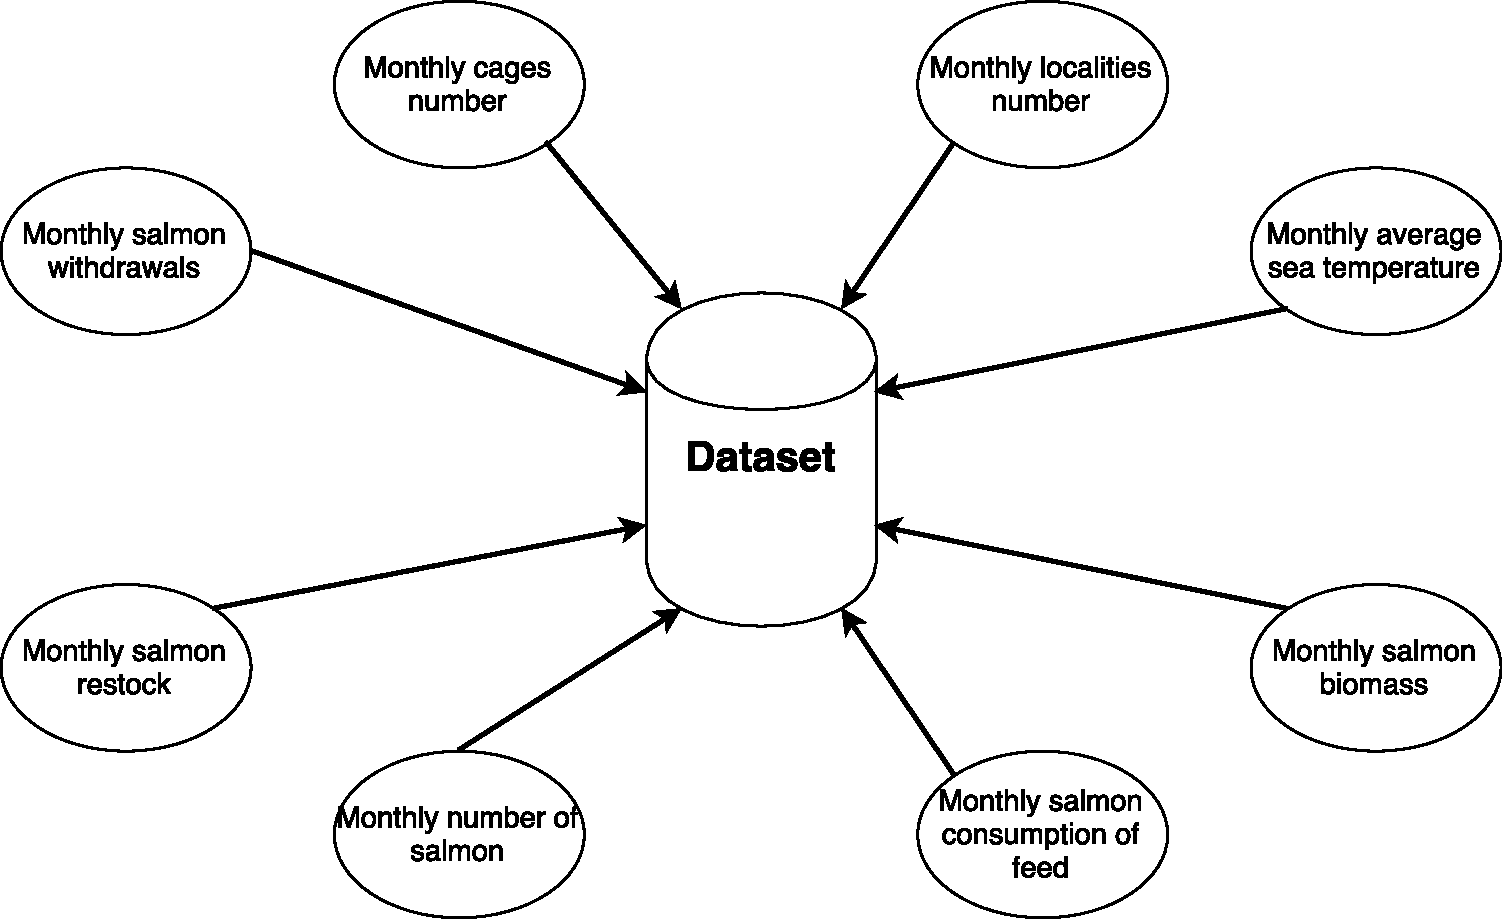
\includegraphics[width=1\textwidth]{Files/Dataset2.pdf}}
    \caption{Dataset structure.}
\end{figure}

\makebox[\textwidth][c]{
\resizebox{1.3\textwidth}{!}{
   \begin{tabular}{ | l | l | l | l | l | l | l |}
            \hline
\textbf{Input}							&	\textbf{Content}	& \textbf{Unit} & \textbf{Frequency} & \textbf{Period} & \textbf{Location} & \textbf{Source}	\\ \hline
1. Cages							&	\multicolumn{1}{p{4cm}|}{\raggedright Reported number of cages with salmon and rainbow trout.}
									& Number & Monthly & January 2007 - December 2014 & Troms & fiskeridir.no	\\ \hline
									
2. Localities						& \multicolumn{1}{p{4cm}|}{\raggedright Reported number of localities with salmon and rainbow trout.}
									& Number & Monthly & January 2007 - December 2014 & Troms & fiskeridir.no	\\ \hline
3. Average Sea Temperature 			& \multicolumn{1}{p{4cm}|}{\raggedright }	
									&  & Monthly &  & Troms & 	\\ \hline
4. Salmon\_consumption\_of\_feed	&  \multicolumn{1}{p{4cm}|}{\raggedright Reported feed consumption for Salmon.}		
									& Tonnes & Monthly & January 2007 - December 2014 & Troms & fiskeridir.no	\\ \hline
5. Salmon\_restock 				& \multicolumn{1}{p{4cm}|}{\raggedright Fish restock reported for Salmon.}	
									& 1000 pcs & Monthly & January 2007 - December 2014 & Troms & fiskeridir.no	\\ \hline
6. Salmon\_withdrawals 			& \multicolumn{1}{p{4cm}|}{\raggedright Withdrawals of Salmon for slaughter. } 		
									& Tonnes & Monthly & January 2007 - December 2014 & Troms & fiskeridir.no	\\ \hline
7. Salmon\_biomass\_end\_month		& \multicolumn{1}{p{4cm}|}{\raggedright Reported biomass of Salmon. }
									& Tonnes & Monthly & January 2007 - December 2014 & Troms & fiskeridir.no	\\ \hline
8. Salmon\_number\_end\_month 		& \multicolumn{1}{p{4cm}|}{\raggedright Reported number of Salmon. }		
									& Number & Monthly & January 2007 - December 2014 & Troms & fiskeridir.no	\\ \hline
    \end{tabular}}}

\newpage


	
	


\part{Data Analysis and Dislaying}
\section{Analysis of the data}
Total implementation link for data analyzer : \\
\url{https://github.com/Sprea22/Data_Analyzer_Python}

During this part the main purpose is to analyze the whole dataset in order to find some kind of useful informations later on. 

The output of this phase will basically be for each single data input:
\begin{itemize}
\item Total graphic of the input data from 2005 to 2016.
\item Graphic of the input data for each single year from 2005 to 2016.
\item Correlation matrix between different months of the same input.
\item Correlation matrix between different years of the same input.
\end{itemize}

And then it also provides:
\begin{itemize}
\item General correlation matrix between all the different inputs.
\item Graphic of the normalized angular coefficients of all the inputs.
\end{itemize}

It's important to remind that this phase can be implemented in different ways and with different programming language;\\
This proceure will describes the system implentation using Python, so be sure to have installed all the necessary for compile and execute Python code on your platform.

Current development environment:\\
Python version: 2.7.12\\
Linux kernel version number: Linux Asus 4.4.0-71-generic SMP\\

The system that it's going to be implemented during this part of the work could be divided in two subsystems:
\begin{itemize}
\item Single Input Analyzer (SIA): Used for analyze a single data input.
\item Multiple Inputs Analyzer (MIA): Used for analyze multiple data inputs.
\end{itemize}
\newpage


\newpage
\subsection{Single Input Analyzer}
It's possible to check out the total implementation code of the SIA in the appendice  [\ref{SIA_Implementation}].
The implementation of this Analyzer can be divided in the following parts:
\begin{itemize}
\item SIA imported libraries. 
\item SIA part I: Generate and display a graphic about current input with total data from 2005 to 2016.
\item SIA part II: Generate and display a graphic about current input for each year from 2005 to 2016.
\item SIA part III: Generate and display a graphic that contains the correlation matrix between each single year from 2005 to 2016 of the current input.
\item SIA part IV: Generate and display a graphic that contains the correlation matrix between each single months of the year of the current input.
\item SIA part V: Generate and display a single overview image for the current input.
\end{itemize}

\subsubsection{SIA: Requirements for reusability}
The system that is going to be implemented in this phase of the work could be used for other data inputs as well, but there are of course some kind of requiriments about the dataset that are necessary for let it works in a proper way.\\
The aalysis system need in input a dataset structure that:
\begin{itemize}
\item Data from January 2005 to December 2016
\item One single value for each month
\end{itemize}
It means that the dataset must contains 144 values for each single input.

\subsubsection{SIA: Imported libraries}
Specific Python libraries have been imported for the implementation of this system.
It's possible to find out a list of this libraries with a specific description for each of them in the appendice [\ref{SIA_libraries}].

\newpage

\subsubsection{SIA section I: Total graphic for all the years}
\textbf{Goal:}\\
Generate and display the total graphic about current input from 2005 to 2016.

\textbf{Requirements:}\\
- Data content: 144 values, 1 value for each month from 2005 to 2016

\textbf{Implementation:}\\
It's possible to check out the full ccommented code in the appendice: [\ref{SIA_section_I}]

\textbf{Results:} \\
With this first part of the code has been reached the first goal of displaying and saving the basic graphic about the current input from 2005 to 2016 with also the relative trendline, that looks like this example:

\begin{figure}[H]
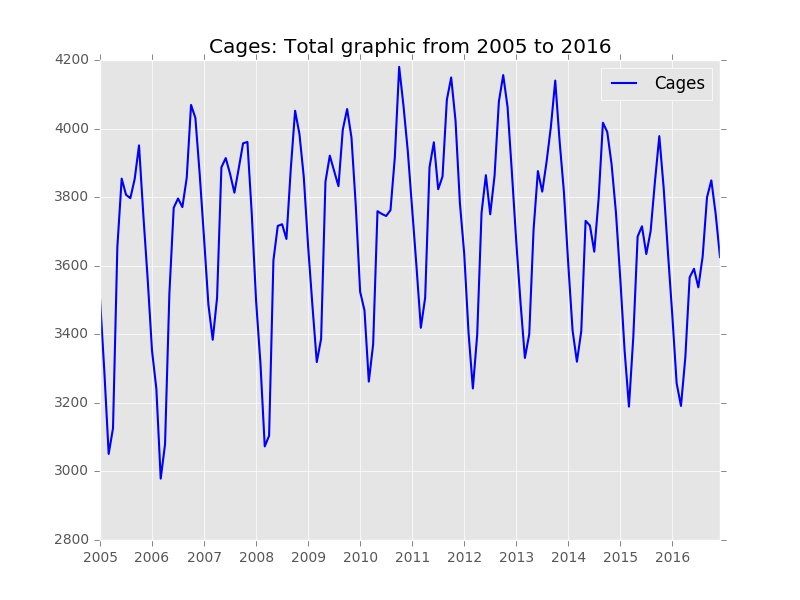
\includegraphics[width=1\textwidth]{Files/Cages_Total.jpg}
\caption{Total graphic about current input with total data from 2005 to 2016.}
\end{figure}



\newpage
\subsubsection{SIA section II: Single graphics for each year}

\textbf{Goal:}\\
Generate and display a graphic that contains the plots of each single year from 2005 to 2016 of the current input. 

\textbf{Requirements:}\\
- Data content: 144 values, 1 value for each month from 2005 to 2016

\textbf{Implementation:}\\
It's possible to check out the full ccommented code in the appendice: [\ref{SIA_section_II}]

\textbf{Results:} \\
With this second part of the code has been reached the goal of displaying and saving the graphic of the plots for each single year of the current input from 2005 to 2016, that looks like this example:

\begin{figure}[H]
	\centering
    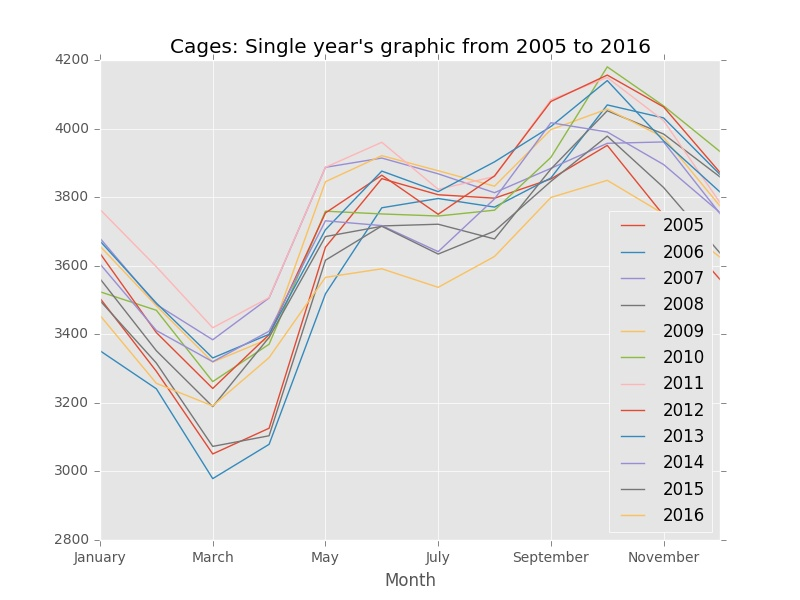
\includegraphics[width=1\textwidth]{Files/Cages_Years.jpg}
    \caption{Graphics for each single year of the input data from 2005 to 2016}
\end{figure}




\newpage
\subsubsection{SIA section III: Correlation matrix between years}

\textbf{Goal:}\\
Calculate the correlation coefficients between each single year from 2005 to 2016 of the current input and then display it with a correlation matrix.

\textbf{Requirements:}\\
- Data content: 144 values, 1 value for each month from 2005 to 2016

\textbf{Implementation:}\\
It's possible to check out the full ccommented code in the appendice: [\ref{SIA_section_III}]

\textbf{Results:} \\
With this part of the code have been calculated the correlation coefficients between each single year from 2005 to 2016 of the current input and saved it in a document. \\
Then has been also displayed and saved the correlation matrix about it, that looks like the current example:

\begin{figure}[H]
	\centering
    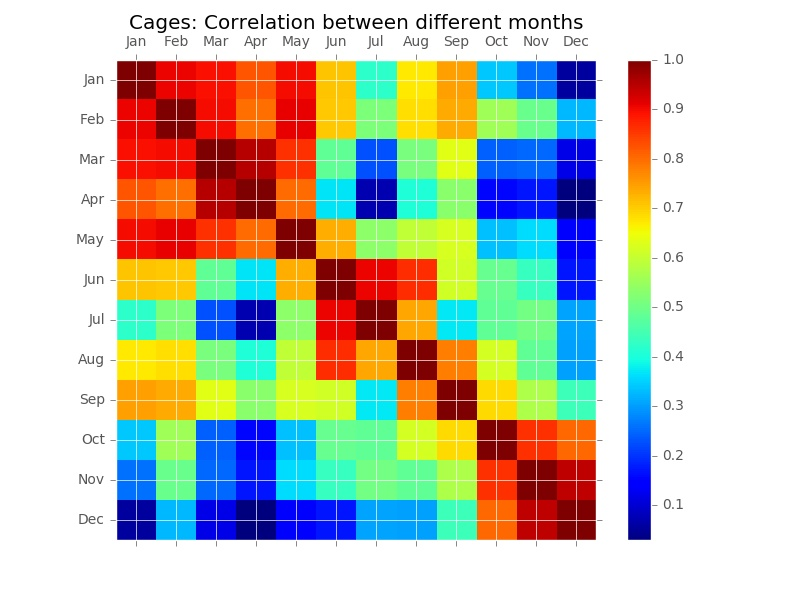
\includegraphics[width=1\textwidth]{Files/Cages_Months_Matrix.jpg}
    \caption{Correlation matrix between different months of the same input}
\end{figure}




\newpage
\subsubsection{SIA section IV: Correlation matrix between months}

\textbf{Goal:}\\
Calculate the correlation coefficients between each single month from 2005 to 2016 of the current input and then display it with a correlation matrix.

\textbf{Requirements:}\\
- Data content: 144 values, 1 value for each month from 2005 to 2016

\textbf{Implementation:}\\
It's possible to check out the full ccommented code in the appendice: [\ref{SIA_section_IV}]


\textbf{Results:} \\
With this part of the code have been calculated the correlation coefficients between each single month from 2005 to 2016 of the current input and saved it in a document. \\
Then has been also displayed and saved the correlation matrix about it, that looks like the current example:

\begin{figure}[H]
	\centering
    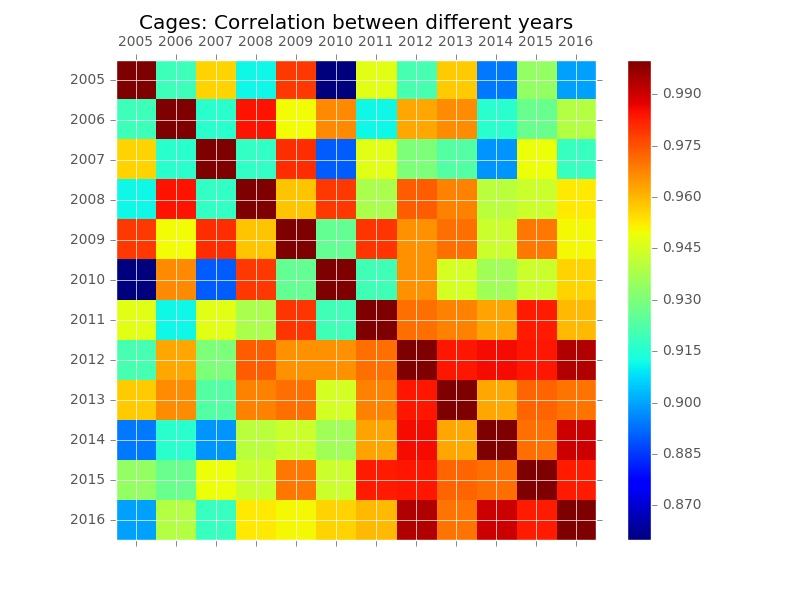
\includegraphics[width=1\textwidth]{Files/Cages_Years_Matrix.jpg}
    \caption{Correlation matrix between different years of the same input}
\end{figure}


\newpage
\subsubsection{SIA section V: Single overview}

\textbf{Goal:}\\
Generate and display a single overview image that contains all the graphics previous calculated for the current input.

\textbf{Implementation:}\\
It's possible to check out the full ccommented code in the appendice: [\ref{SIA_section_V}]

\textbf{Requirements:}\\
- All the graphics about the current input have to be already calculated and saved.

\textbf{Results:}
With this part of the code it's possible to have a single overview image for the current input, that is basically showing and comparing all the graphics that have already been calculated about this input. It looks like this example:
\begin{figure}[H]
    \makebox[\textwidth][c]{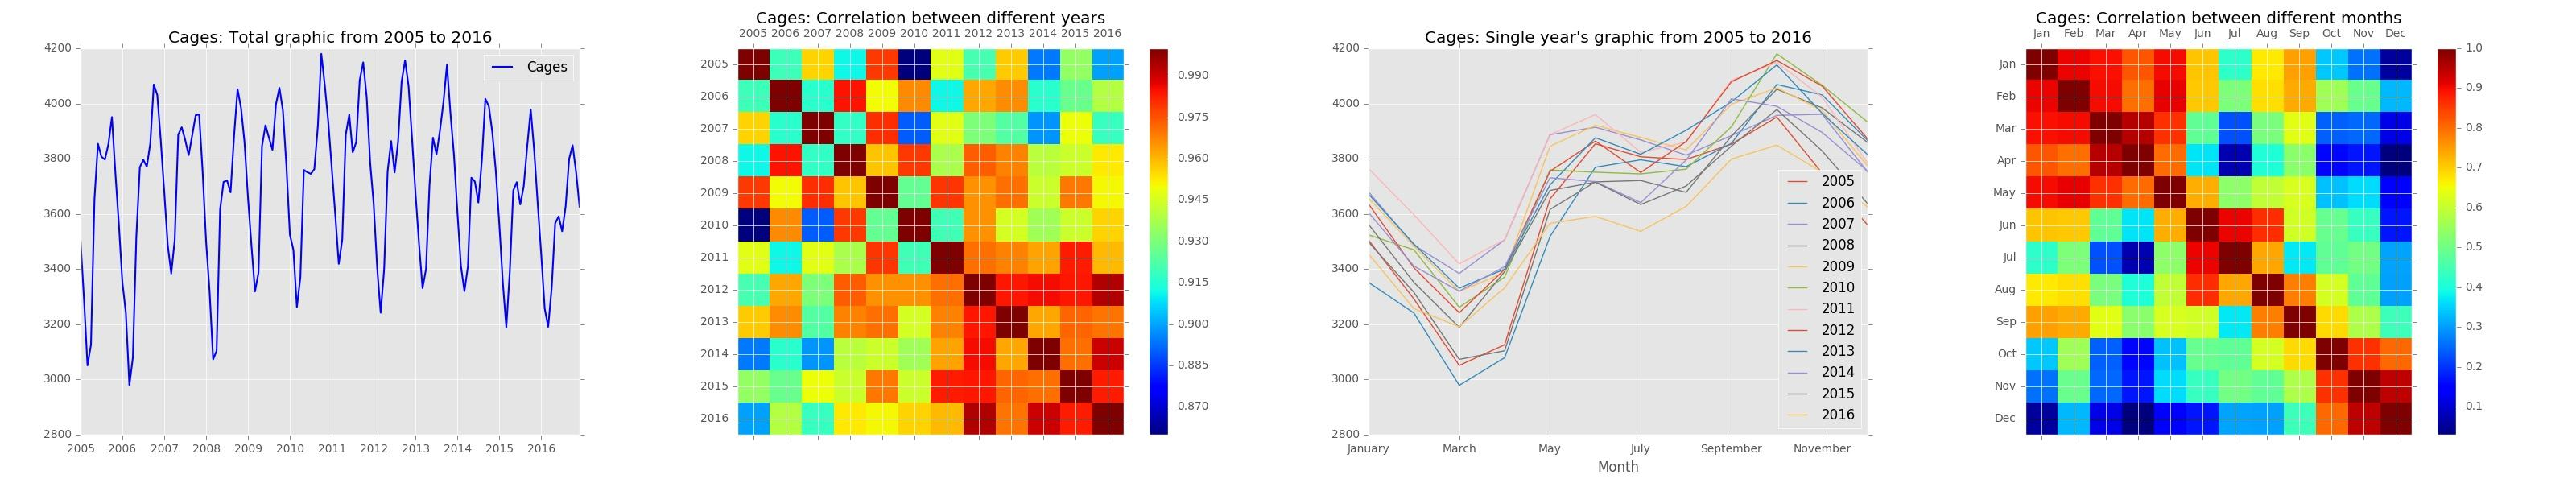
\includegraphics[width=1.4\textwidth]{Files/Cages_Overview.jpg}}
    \caption{Example of "Single Input Overview Image"}
\end{figure}

\newpage

\subsection{Multiple Inputs Analyzer}
\subsubsection{MIA: Requirements for reusability}
The system that is going to be implemented during this phase it's not reusable at all.
It means that has been implemented just for analyze and display the result about the dataset that is used during this work.

\subsubsection{SIA: Imported libraries}
Specific Python libraries have been imported for the implementation of this system.
It's possible to find out a list of this libraries with a specific description for each of them in the appendice [\ref{MIA_Libraries}].

\newpage

\subsubsection{MIA: Implementation}
\textbf{Goal:}\\
This analyzer is mainly used for show the correlation coefficent between the diffent inputs along the total period (from 2005 o 2016) and also for display the comparison between the normalized angular coefficients for each single input in the current dataset.

\textbf{Requirements:}\\
How it's written above, this part of the system is not reusable at all.\\
So the requirements are strict about the input data, that have to be exactly tha same that we are using during this work.\\
Of course this system can be used for the other dataset, but before doing it you have to personalize the implementation code.

\textbf{Implementation:}\\
It's possible to check out the full ccommented code in the appendice: [\ref{MIA_Implementation}]

\textbf{Results:} \\
The first part of the MIA implementation allows to calculate the correlation coefficients value between each single inputs and then also to display and save it. The graphic result looks like:

\begin{figure}[H]
	\centering
    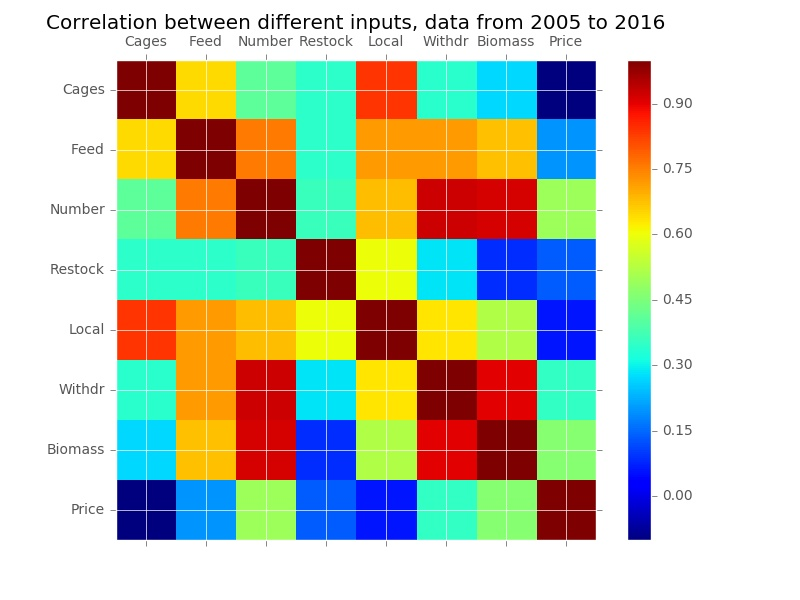
\includegraphics[width=0.90\textwidth]{Files/Total_Dataset_Years_Matrix.jpg}
    \caption{Correlation matrix between different inputs with data from 2005 to 2016.}
\end{figure}

\newpage

The second part of the MIA implementation allows to display a graphic that compare the normalized angular coefficients for each single input that have been already calculated and reported in a document. The result graphic look like:

\begin{figure}[H]
	\centering
    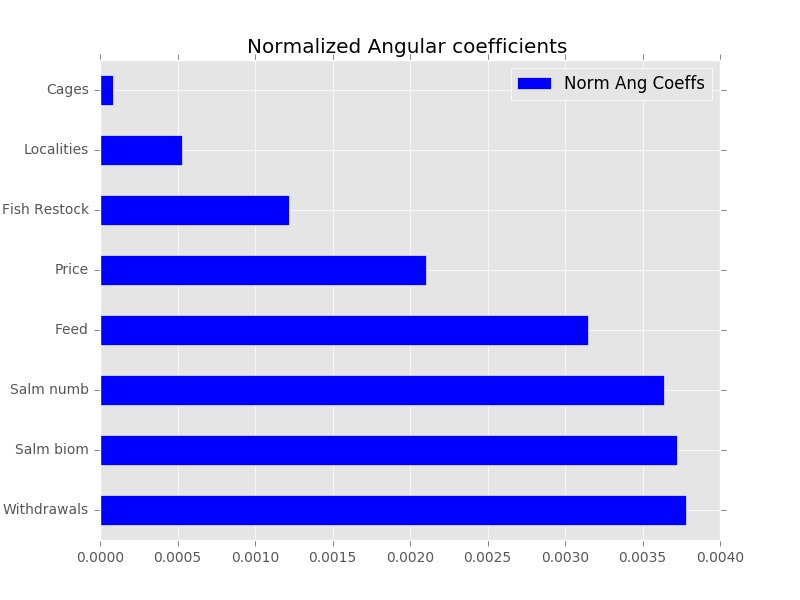
\includegraphics[width=0.90\textwidth]{Files/Norm_Ang_Coeffs.jpg}
    \caption{Normalized angular coefficients of each input's trendline.}
\end{figure}


\newpage
\section{Extract information from data}
 % Data Analysis and Displaying

\part{Data Prediction}
\section{Prediction of values about the data}

Some basic and general goals were defined before starting this phase, with the idea of "doing more if it's possible". Basically the main purpose was the one of, after the previous analysis, predict some values and evaluate the quality of the results.
This prediction system was not defined with some specific requirements, so the first main problem was to find a reliable, accurated and user-friendly way to predict and display prediction of values.

Since the current dataset can be considered like a time series, in this phase we will develop the data prediction system using an ARIMA machine implemented in python.

The ARIMA machine can be configured with several configurations, it allows you to have more accurated results; so the first thing was to find the right configuration of the ARIMA machine of each single input which we are interested to forecast.

During this phase of the work have been implemented 3 different subsystems for different purposes:
\begin{enumerate}
\item Evaluating System
\item Training System
\item Future Prediction System
\end{enumerate}

\newpage
\subsection{Evaluating System}
\textbf{Goal:}\\ 
Used for evaluate different configurations of ARIMA machine. \\ 
It tests 112 different configurations for each single input that we would like to forecast and report the results with each MAPE (Mean Average Percentage Error) values.

\textbf{Requirements:}\\
There are not strict requirements needed. There are no type of restriction neither about the length or about the type of data.

\textbf{Code implementation:}\\
The most important part of the code about the Evaluating System is the following.\\
Basically the method ARIMA() allows to train a model based on historic values (history) and a specific order (p,d,q). After that it's possible to call the method forecast() through the trained model and having some predictions like result.
\begin{lstlisting}
model = ARIMA(history, order=arima_order)
model_fit = model.fit(disp=0)
yhat = model_fit.forecast()[0]
\end{lstlisting}

This system will provide 112 different ARIMA configurations results for each single input, and in particular it will display the best ARIMA configuration, that is the one with the lower MAPE.

\textbf{Results:}\\
The system will display the MAPE between real value and predicted values for each single tested ARIMA machine, in particular the configuration that gives the best result.
All these results have been reported in a document and then also displayed with a 3D graphic that allows to see the MAPE value for each different order in input.



\begin{figure}[H]
	\raggedleft
	\makebox[\textwidth][c]{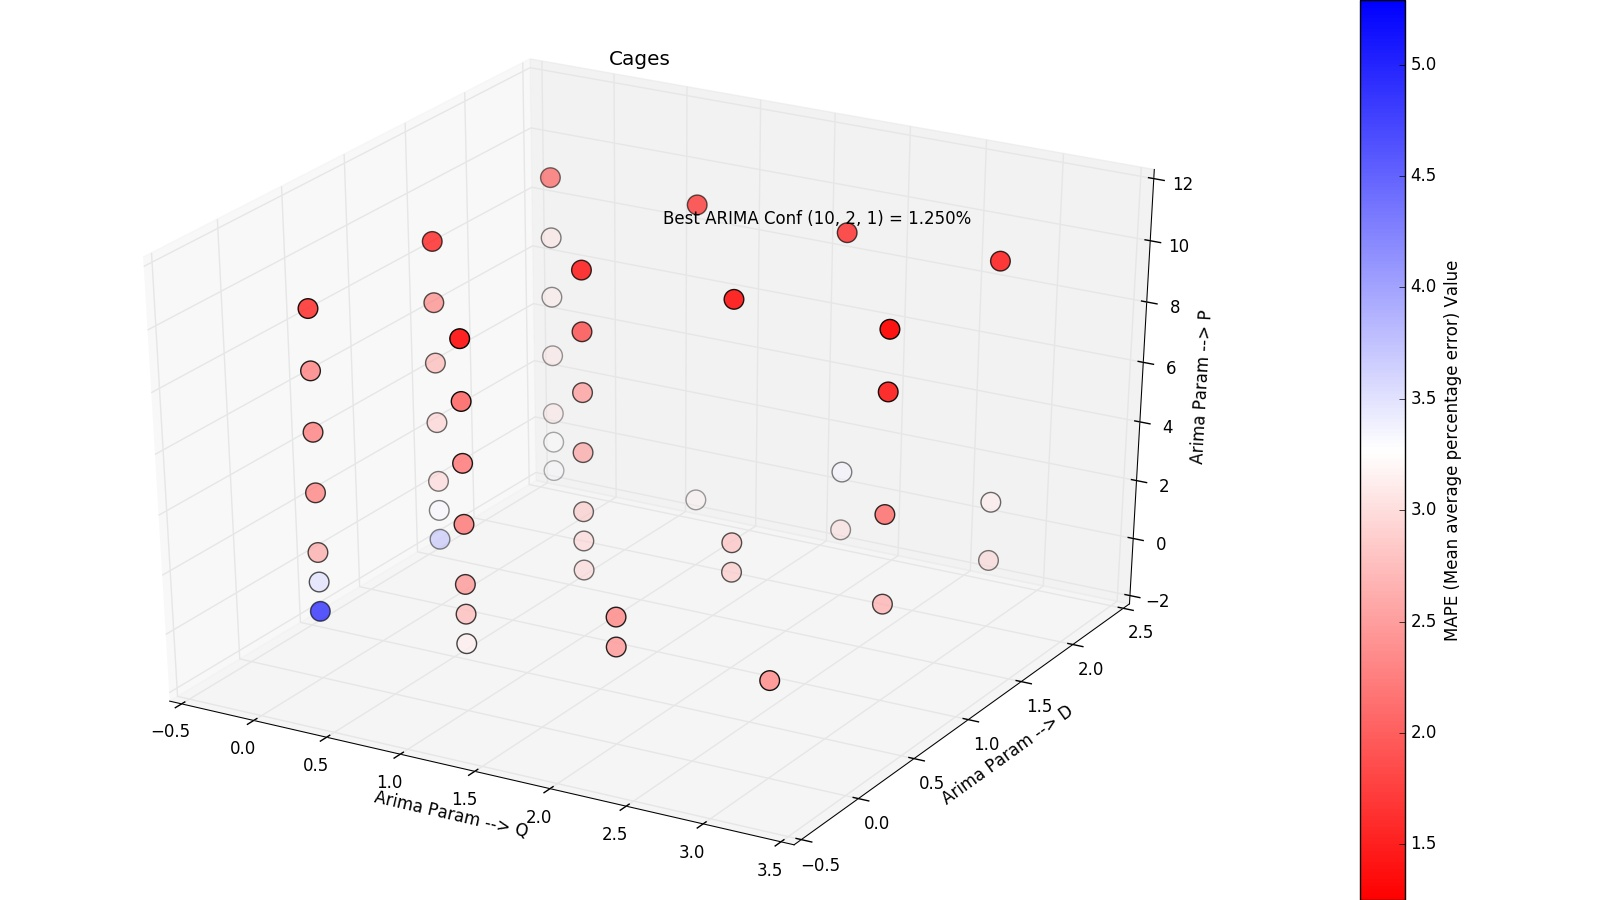
\includegraphics[width=0.7\textwidth]{Files/Cages_MAPE.jpg}}
    \caption{Graphic that displays different MAPE values for each ARIMA order.}
\end{figure}

 
 
\newpage
\subsection{Training System}
\textbf{Goal:}\\ 
This system has the goal of training/testing a particular specific ARIMA configuration about a data input, and see how much accurate it is. \\


\textbf{Requirements:}\\
Since this Traning System has been used mainly for train and test the current dataset, it need to have like input a dataset that follows the same format:
- Data content: 144 values, 1 value for each month from 2005 to 2016

\textbf{Code implementation:}\\
First of all this system it's going to split the input data in two part:\\
- Train data: values which the ARIMA model is going to use for training. \\
- Test data: values which are hided by the forecasting model. \\
Once the ARIMA model has been created, the system will try to predict the future values, that are actually the "Test data".\\
Once the predictions have been calculated it's possible to display the "Test data" (that are the real values) and the predicted values, just to see how much the ARIMA configuration is accurate.
\begin{lstlisting}
model = ARIMA(history, order=arima_order)
model_fit = model.fit(disp=0)
yhat = model_fit.forecast()[0]
\end{lstlisting}
\begin{lstlisting}
series = pd.read_csv("Dataset.csv", usecols=[sys.argv[1]])
series.plot(color="blue", linewidth=1.5,
		 label="Series: "+sys.argv[1])


output = Series.from_csv('Output_Files/predictions.csv')
output.plot(color="red", linewidth=1.5,
		label="Prediction test:")
\end{lstlisting}
\textbf{Results:}\\

\begin{figure}[H]
	\centering
    \makebox[\textwidth][c]{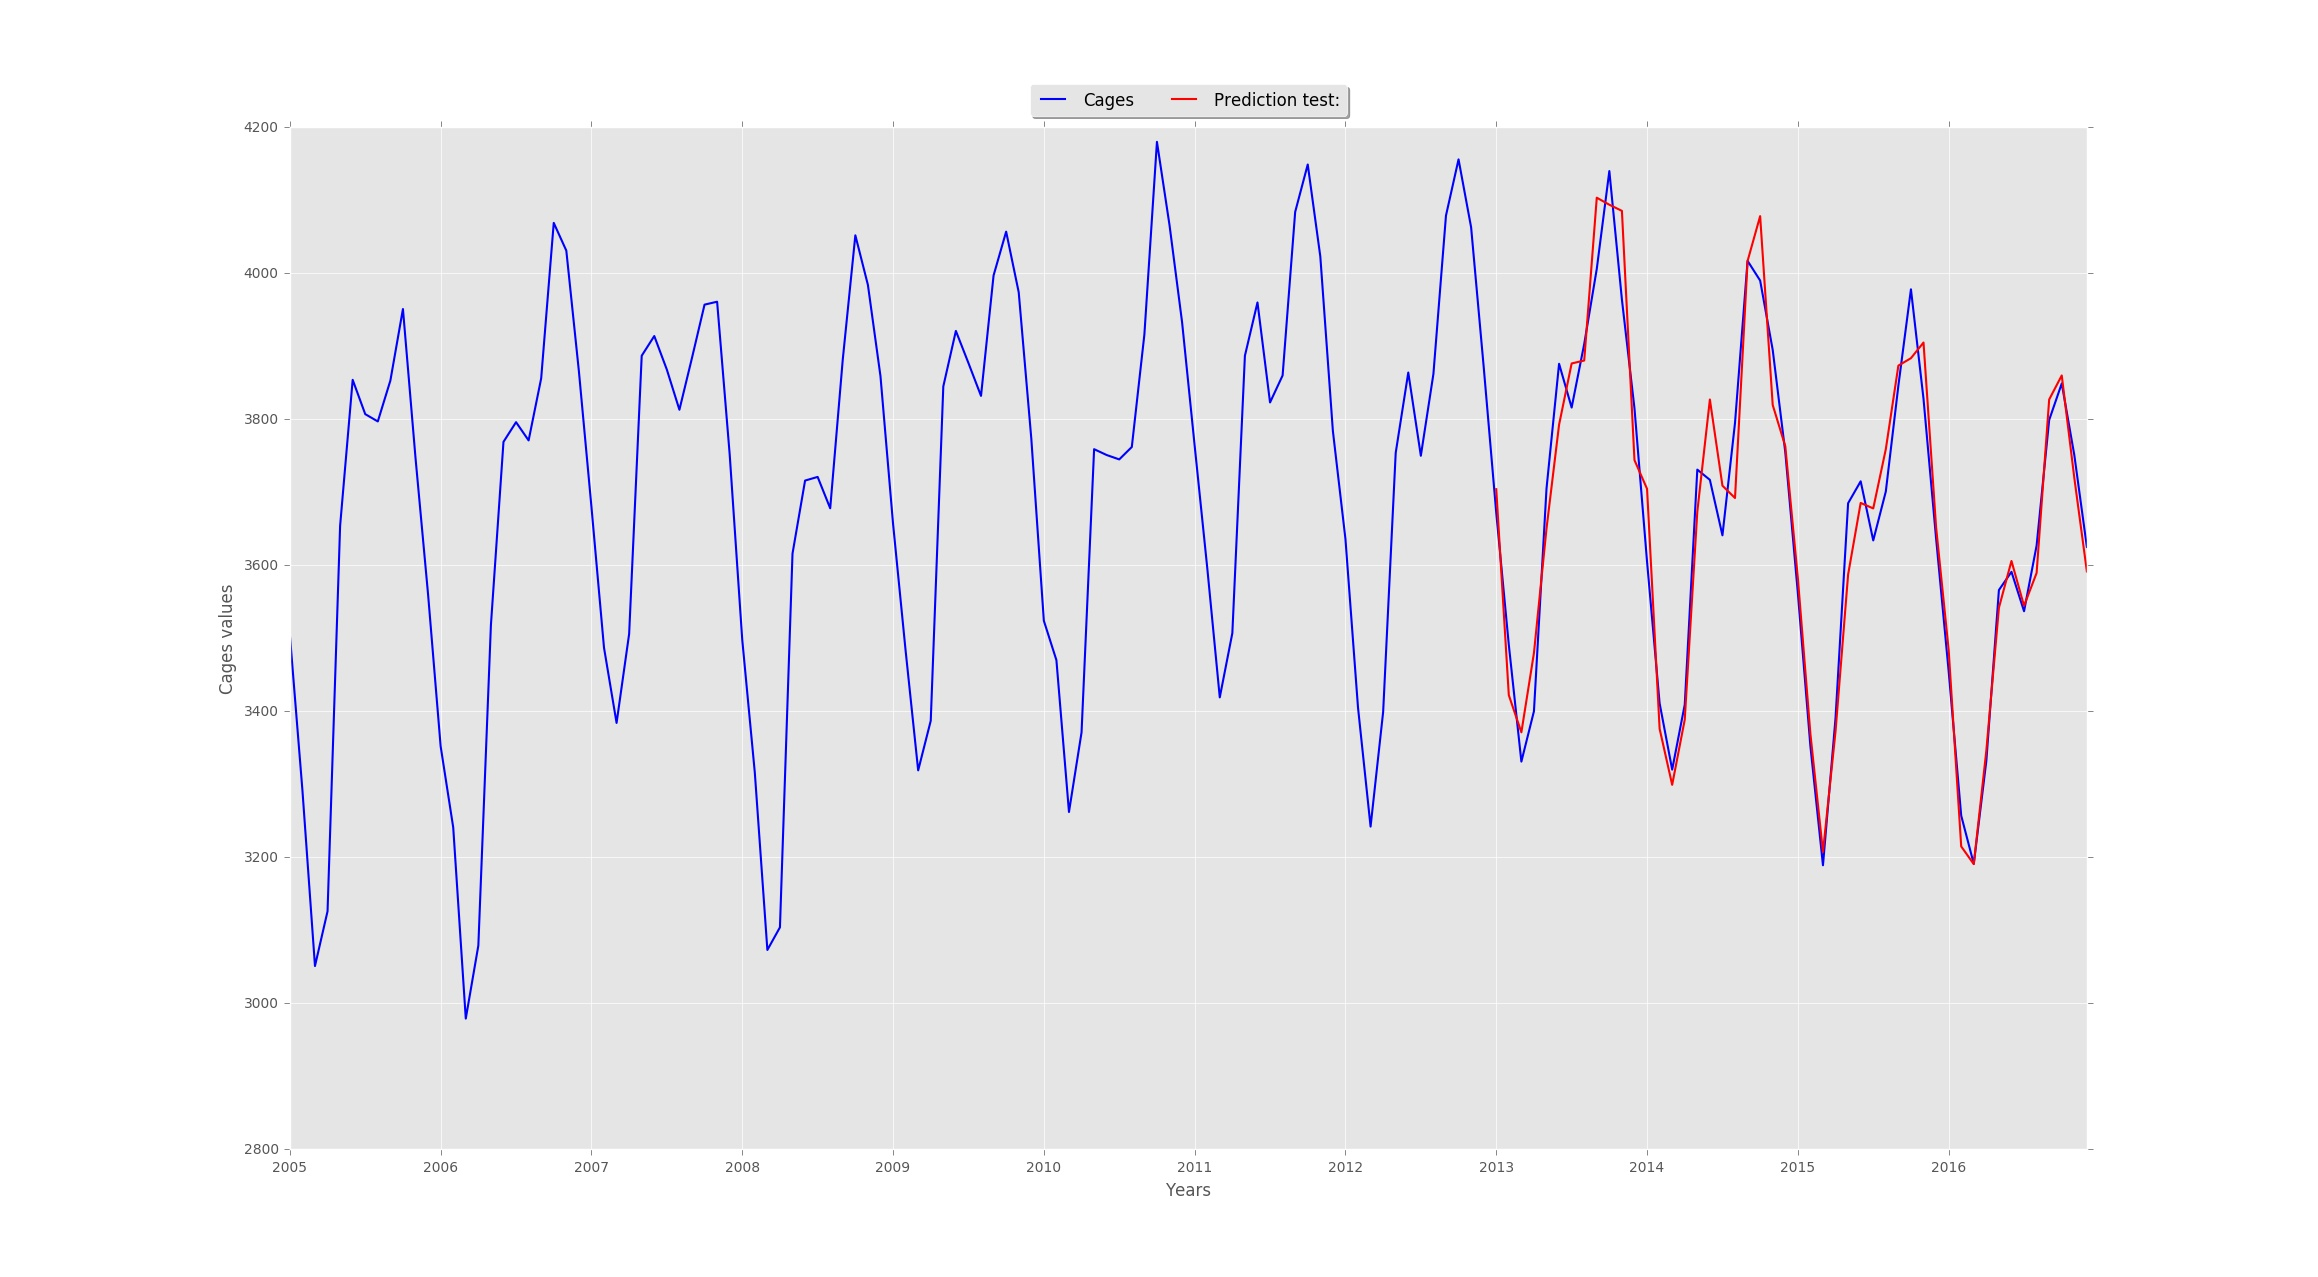
\includegraphics[width=1.5\textwidth]{Files/Cages_TRAIN.jpg}}
    \caption{Graphic that displays the predicted values from a particular ARIMA machine configuration and the historic real values.}
\end{figure}


\newpage
\subsection{Future Prediction System}
\textbf{Goal:}\\ 
This part of the work has the goal of display some real prediction of values in the future. \\
It basically collects real future values, in this particular are values about 2017, of each single input and then, once calculated also the prediction values, it's going to display on the same graphic:\\
- Historic values\\
- Predicted future values\\
- Real values (if are available)

\textbf{Requirements:}\\
This system has to be as much reusable as possible, so there are not that strict requirements. You can reuse this Future Prediction System with any kind of dataset with no restrictions about length. \\
The only requirement to let it works in a proper way is that you have to set the historic and real values datasets in the right way; it means that you have to write down the historic values in the dataset in this way:

Index | Input\\
1	  |	Value1\\
2	  |	Value2\\
3	  |	Value3\\
..	  |	..\\
120	  |	Value120\\
121	  |	Value121\\
122   |	Value122\\

And then, if you want to compare the predicted values with some real values that are already available, you have to set the real values dataset in this way:

Index | Input\\
123	  |	Value123\\
124	  |	Value124\\
125	  |	Value125\\
126	  |	\\
127	  |	\\
128   |	\\

\textbf{Code implementation:}\\
\begin{lstlisting}
model = ARIMA(history, order=arima_order)
model_fit = model.fit(disp=0)
yhat = model_fit.forecast()[0]
\end{lstlisting}


\begin{lstlisting}
# 1) Historic values
series = pd.read_csv("HISTORIC DATASET", 
			usecols=[sys.argv[1]])
series.plot(color="blue",linewidth=1.5)

# 2) Predicted future values
series = Series.from_csv("PREDICTIONS DATASET")
series.plot(color="red", linewidth=1.5, 
			label="Prediction Results")

# 3) Real future values
series = pd.read_csv("REAL VALUES DATASET")
pyplot.plot(series["Index"], series[sys.argv[1]],
	color="green", linewidth=1.5, label="Real values")

\end{lstlisting}
\textbf{Results:}\\
The system implemented during this phase allows to predict future for as many months as you want in the future and to display it, compared also with the historic values and real values once are available.
\begin{figure}[H]
	\centering
    \makebox[\textwidth][c]{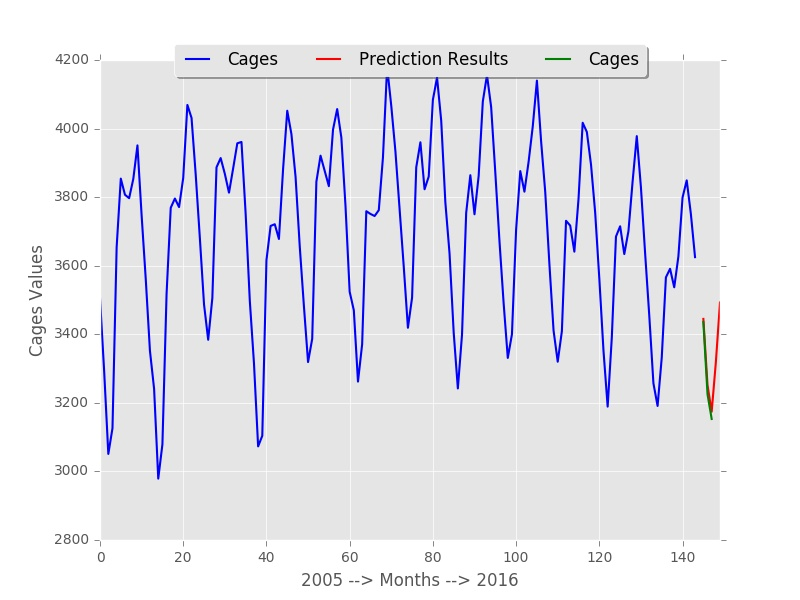
\includegraphics[width=0.5\textwidth]{Files/Cages_Predictions.jpg}}
    \caption{Graphic that display historic, future and predicted values of a input.}
\end{figure}

\newpage

\section{Requirements for reusability}
The subsystems implemented during this phase of the work are almost completely reusable.\\
The reusability this systems allows to get some prediction of values about different kind of dataset, in particular:
\begin{itemize}
\item The "Evaluating System" is actually 100\% reusable, and you can use it for evaluate any kind of dataset.
\item The "Future Prediction System" is completely reusable as well, you should only modify the historic values and the real values inside the dataset for it works in a proper way.
\item The "Training System" has been implemented for testing the current dataset, so it's not completely reusable but could be changed very easily and let it works also for other data input.
\end{itemize}


 % Data Prediction

\part{Future Works}
\section{Dataset about single locality}
This thesis allows to have a general overview and predictions of values about the aquaculture business in Norway. 

But it would be much more useful, in particular for people into the aquaculture business, to use this system to have an overview and predictions of data provided by a single locality of aquaculture.\\
In this case the system could be used from the owner of the locality to analyze historic values and use the prediction system to have a forecast about some particular parameters.

\section{Visualization of the data}

\section{Test prediction system with a bigger dataset}

\newpage

\section{Prediction system as a service}
This system has been developed with the idea that it could become a "Service system", that is basically a configuration of technology and organizational networks designed to deliver services that satisfy the needs or wants of customers.
Since the prediction system implemented during this work is almost 100\% reusable, it could be used from people for prediction about any kind of data. 

Basically the idea is to create a web application that allows to let you upload your own dataset, choose your own preferences and prediction settings, and then the system will calculate and display prediction of the current values in the future together with the MAPE (Mean Average Percentage Error) to have an idea bout how accurate are the.\\


\begin{figure}[H]
	\centering
        \makebox[\textwidth][c]{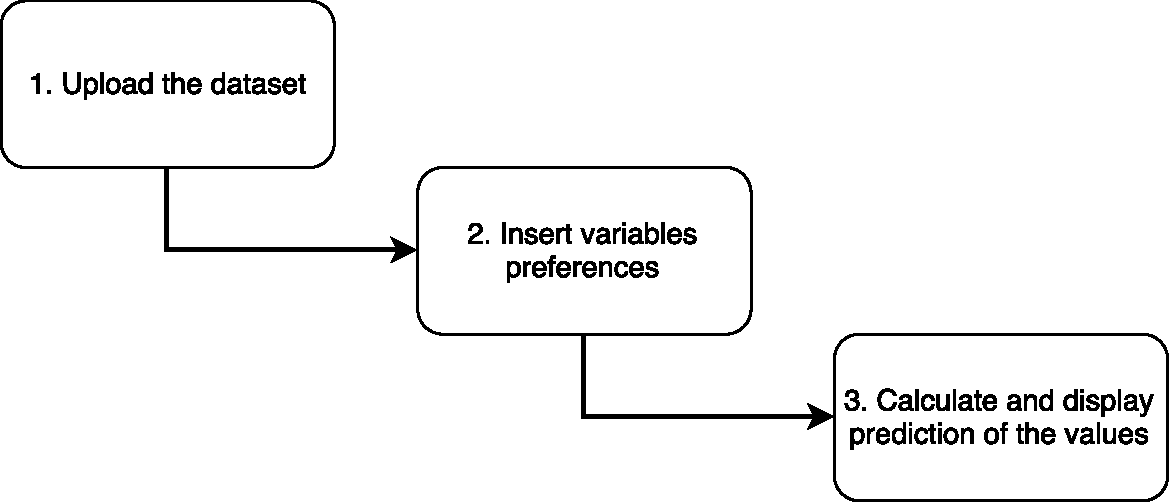
\includegraphics[width=1\textwidth]{Files/ServiceSystem.pdf}}
    \caption{Idea of the Servie System for predictions.}
\end{figure}






